\chapter{Méthode + Théorie}

\section{Structure d'une protéine et d'un complexe}

L'objectif du projet étant de modéliser l'interface de contact entre deux protéines,
il est important de comprendre la structure d'une protéine. Nous verrons également
comment sont stockées ces structures, grâce au fichiers \textit{.pdb}.

\subsection*{Structure}

Les protéines sont des molécules biologiques présentes dans toutes les cellules vivantes.
Elles sont constituées d'un enchaînement d'acides aminés \cite{Prot}.
Les protéines assurent diverses fonctions au sein de la cellule vivante et dans les tissus.
Elles peuvent avoir un rôle enzymatique, structurel, permettre la mobilité des molécules, la
régulation de l'expression génétique ou encore transmettre des signaux cellulaires.
Les chaînes protéiques constituant les protéines sont synthétisées dans la cellule. Le
matériel génétique de la cellule détermine l'ordre d'enchaînement des acides aminés.
Les protéines adoptent alors une structure en trois dimensions qui leur permet d'assurer
 leur fonction biologique. Les protéines peuvent interagir ensemble afin d'assurer certaines
fonctions biologiques. Ces interactions forment des complexes protéiques. Les structures
 des protéines et leurs interactions sont particulièrement utilisées en chimie médicinale.
L'étude des surfaces et des espaces disponibles peut guider la recherche d'un nouveau
médicament. La cristallographie est utilisée pour étudier la structure des protéines à
l'échelle atomique. Elle s'appuie sur le phénomène physique de diffraction des ondes
électromagnétiques (rayons X).

Le complexe que nous étudions dans ce projet est l'interaction entre
deux protéines. La structure de ce complexe peut être analysée en étudiant l'interface
entre les deux protéines le composant. On comprend dès lors que modéliser cette interface
pour la visualiser peut avoir une importance cruciale en recherche biologique et médicinale.

\subsection*{Fichier de stockage}

Les données utilisables d'une protéine (ou d'un complexe) sont stockées grâce aux
fichiers \textit{.pdb} (voir figure \ref{fig::pdb_file}). Ces fichiers, leur lecture et l'interprétation des données
qu'ils contiennent, sont essentiels à l'observation des protéines. En effet, chaque
ligne, exceptée la première, correspond à un atome composant la protéine étudiée.
Ces lignes contiennent des informations telles que la chaîne à laquelle appartient
l'atome, son acide aminé ou ses coordonnées dans l'espace (en $\si{\angstrom}$).

\begin{figure}[ht]
  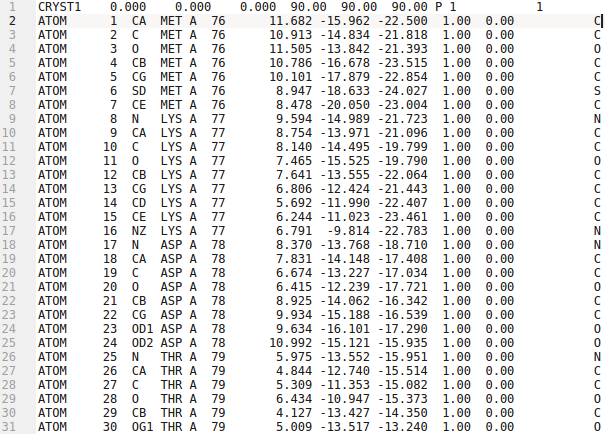
\includegraphics[width=\textwidth]{figures/pdb_example.png}
  \caption{Exemple de fichier .pdb}
  \label{fig::pdb_file}
\end{figure}

Dans la suite du projet, nous considérerons que les atomes sont des points de l'espace
de masses identiques. Dans un premier temps, les coordonnées des atomes seront extraites.
Le nuage de point obtenu constitue la base sur laquelle la méthode de détermination
de l'interface va s'appuyer. Il est donc crucial d'obtenir du fichier \textit{.pdb} un jeu
de données valide et utilisable par le programme implémenté ensuite. Nous verrons également
que d'autres informations, telles que la chaîne (A ou B, colonne 5 de la figure
\ref{fig::pdb_file}), jouent un rôle prépondérant dans le bon fonctionnement du
programme. L'objectif est donc d'extraire un nuage de points cohérent (modélisant
le complexe), pour lui appliquer la triangulation de Delaunay.



\section{Triangulation de Delaunay}

Une protéine est donc représentée comme un nuage de points où chacun de ces points
représente un atome de la protéine. Dans le but d'optimiser les temps de parcours dans
ce nuage de points et de modéliser l'interface entre les deux protéines,
 on utilise la triangulation de Delaunay \cite{Triangulation}.

 Cette triangulation est unique et peut être expliquée de la manière suivante :
 chaque cercle circonscrit à un triangle du nuage de point ne contient que les points
 dudit triangle (voir figure \ref{fig::explication_delaunay}).
 Nous expliquerons dans un premier
 temps la méthode pour déterminer l'interface en deux dimensions avant de la transposer à la
 dimension 3.

\begin{figure}[ht]
\centering
  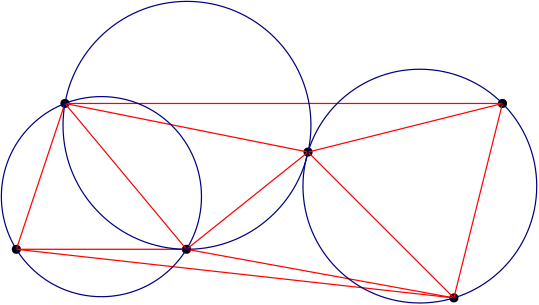
\includegraphics[width=\textwidth]{figures/explication_delaunay.png}
  \caption{Triangulation de Delaunay}
  \label{fig::explication_delaunay}
\end{figure}

\subsection*{Dimension 2}

Il faut appliquer cette triangulation au complexe dont on veut déterminer l'interface, c'est-à dire
aux points donnés par les coordonnées des atomes qui composent le complexe
(voir figure \ref{fig::delaunay_tr}). Les protéines du complexe sont différenciées
par leur couleur (rouge et bleu) sur le schéma. Nous sélectionnons alors la partie utile de
cette triangulation (voir figure \ref{fig::delaunay_reduced}) : nous ne gardons que
les triangles qui contiennent au moins un point à l'interface.
Un point est à l'interface s'il appartient à un triangle contenant au moins un point
de chaque protéine. Le fait de réduire la taille de la triangulation sera utile par la suite
pour accélérer les temps de traitement et de récupération de données concernant l'interface.



\begin{figure}[ht]
\centering
\begin{subfigure}{0.4\textwidth}
  \centering
  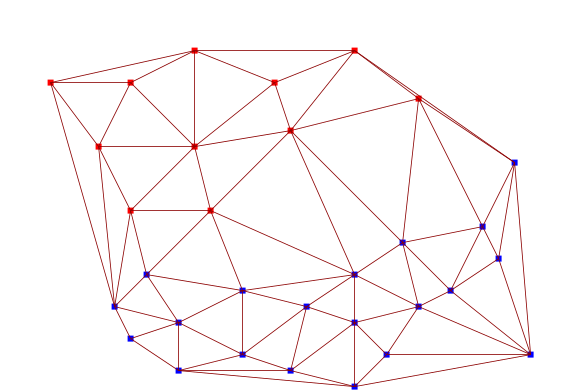
\includegraphics[width=\textwidth]{figures/delaunay.png}
  \caption{Triangulation de Delaunay}
  \label{fig::delaunay_tr}
\end{subfigure}%
\begin{subfigure}{0.2\textwidth}
  \centering
  $\Longrightarrow$
\end{subfigure}%
\begin{subfigure}{0.4\textwidth}
  \centering
  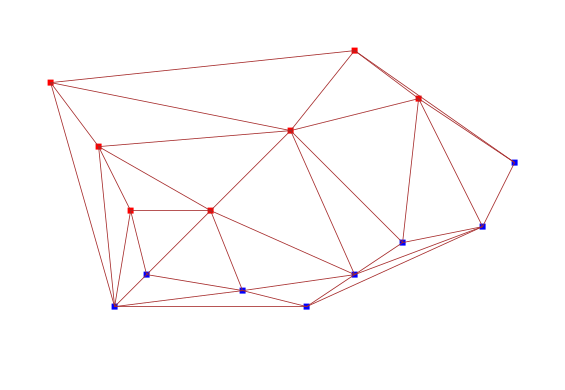
\includegraphics[width=\textwidth]{figures/delaunay_reduced.png}
  \caption{Triangulation réduite}
  \label{fig::delaunay_reduced}
\end{subfigure}
\caption{Réduction d'une triangulation}
\label{fig::delaunays}
\end{figure}

Nous nous intéressons maintenant à la détermination de l'interface, proprement dite.
En ne gardant que les arêtes utiles (voir figure \ref{fig::delaunays_process_1}),
c'est-à-dire celles reliant deux points appartenant
à deux protéines différentes, nous pouvons approximer l'interface de contact grâce
au diagramme de Voronoï.

\begin{figure}[ht]
\centering
\begin{subfigure}{0.45\textwidth}
  \centering
  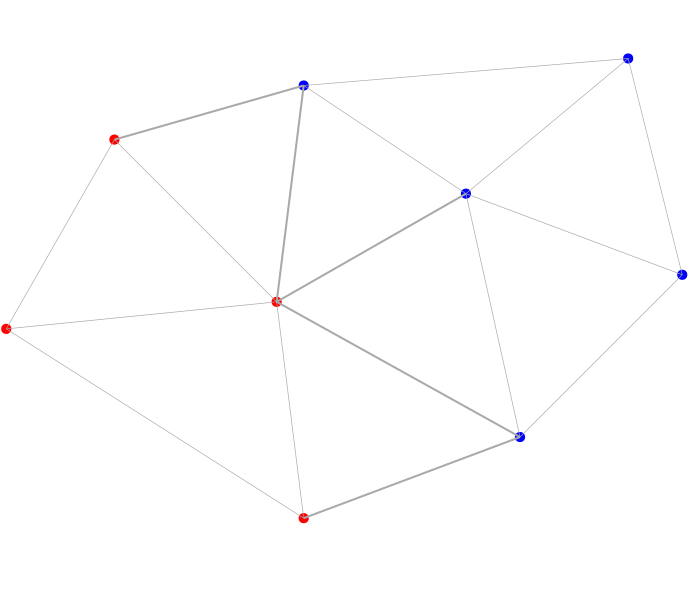
\includegraphics[width=\textwidth]{figures/process_d_1.png}
  \caption{Triangulation de Delaunay}
  \label{fig::process_d_1}
\end{subfigure}%
\begin{subfigure}{0.1\textwidth}
  \centering
  $\Longrightarrow$
\end{subfigure}%
\begin{subfigure}{0.45\textwidth}
  \centering
  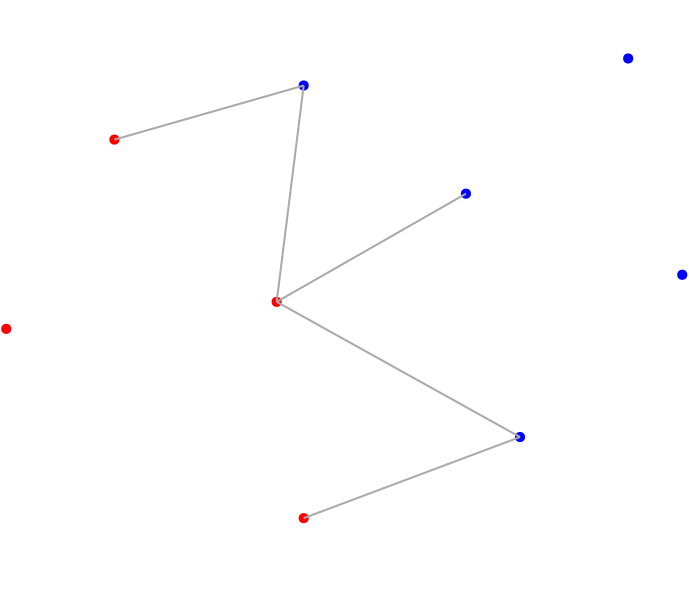
\includegraphics[width=\textwidth]{figures/process_d_2.png}
  \caption{Arêtes à l'interface}
  \label{fig::process_d_2}
\end{subfigure}
\caption{Triangulations et zone utile}
\label{fig::delaunays_process_1}
\end{figure}


Ce diagramme est le dual de la triangulation de Delaunay. Il est representé par les
médiatrices des segments qui constitue la triangulation.
 Il contient donc l'ensemble des points à
égale distance des points de la triangulation (voir figure \ref{fig::process_d_3}).
On ne garde que les parties du diagramme de Voronoï qui correspondent aux arêtes sélectionnées
précédemment, c'est-à-dire les segments du diagramme de Voronoï qui intersectent
avec les arêtes de la triangulation de Delaunay (voir figure \ref{fig::process_d_4}).
Nous obtenons alors une droite par morceaux
qui approxime l'interface de contact en dimension 2.

\begin{figure}[ht]
\centering
\begin{subfigure}{0.45\textwidth}
  \centering
  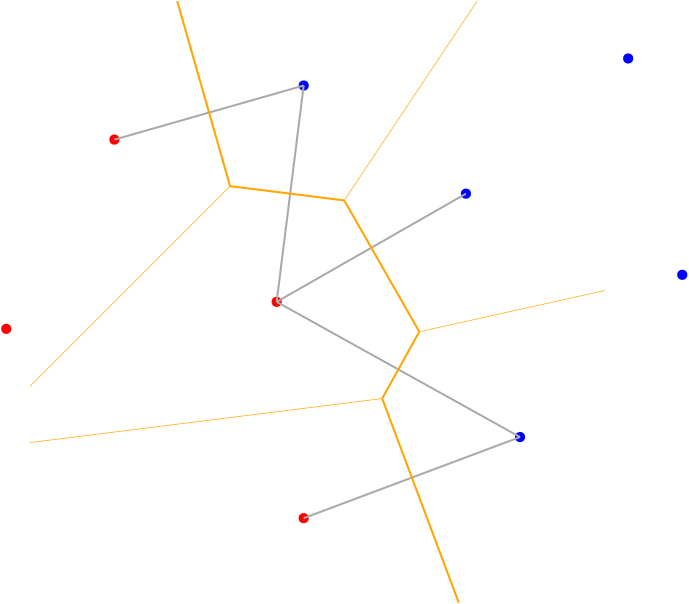
\includegraphics[width=\textwidth]{figures/process_d_3.png}
  \caption{Diagramme de Voronoï}
  \label{fig::process_d_3}
\end{subfigure}%
\begin{subfigure}{0.1\textwidth}
  \centering
  $\Longrightarrow$
\end{subfigure}%
\begin{subfigure}{0.45\textwidth}
  \centering
  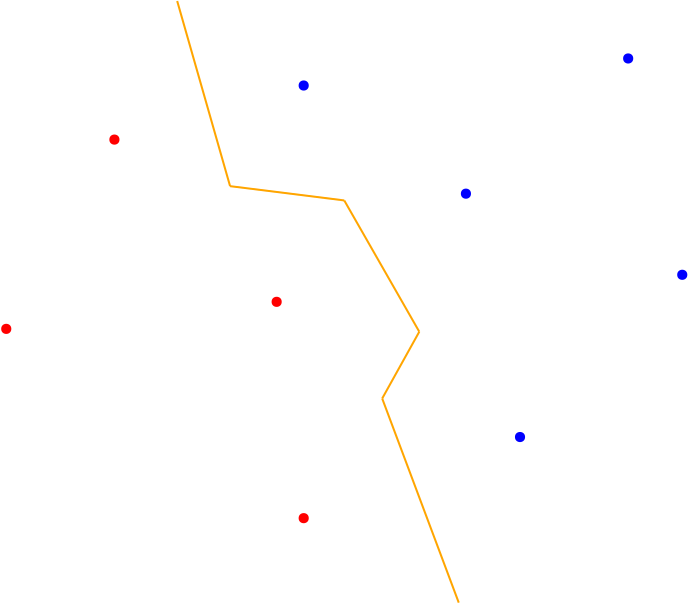
\includegraphics[width=\textwidth]{figures/process_d_4.png}
  \caption{Interface}
  \label{fig::process_d_4}
\end{subfigure}
\caption{Recherche de la surface de contact}
\label{fig::delaunays_process_2}
\end{figure}


\subsection*{Dimension 3}

Si nous transposons la méthode vue ci-dessus en dimension 3, les triangles formés
par les points deviennent des tetrahèdres sur lesquels nous travaillerons pour vérifier
les zones utiles au calcul de l'interface. De la même manière, un tétrahèdre sera considéré
à l'interface s'il contient au moins un atome de chaque protéine.
De plus, le dual d'une arête devient une surface entourant cette arête (voir figure
 \ref{fig::dual_3d}). En rassemblant ces morceaux
de surface, nous obtenons une surface en trois dimensions qui modélise la surface
de contact entre les deux protéines du complexe étudié.

\begin{figure}[ht]
\centering
  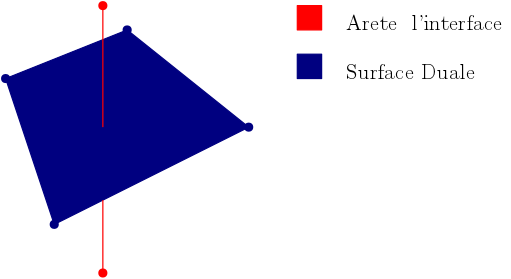
\includegraphics[width=\textwidth]{figures/dual_3d.png}
  \caption{Dual d'une arête en Dimension 3}
  \label{fig::dual_3d}
\end{figure}

La triangulation en trois dimensions d'un nuage de points correspondants aux atomes
d'un complexe donne la figure \ref{fig::delaunays_3d}.

\begin{figure}[ht]
\centering
\begin{subfigure}{0.45\textwidth}
  \centering
  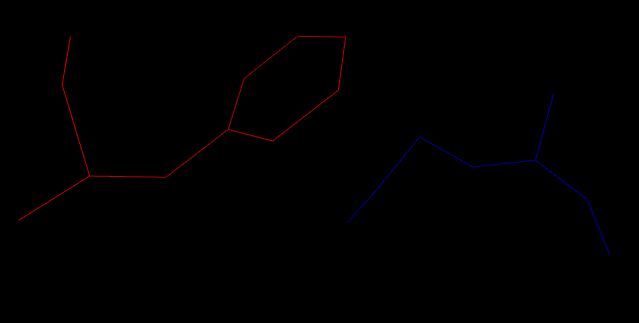
\includegraphics[width=\textwidth]{figures/small_prot.png}
  \caption{Partie d'un complexe}
  \label{fig::small_prot}
\end{subfigure}%
\begin{subfigure}{0.1\textwidth}
  \centering
  $\Longrightarrow$
\end{subfigure}%
\begin{subfigure}{0.45\textwidth}
  \centering
  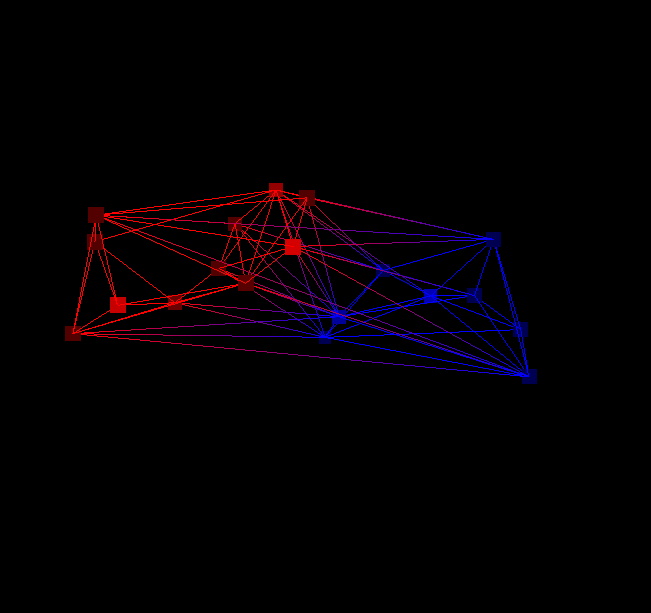
\includegraphics[width=\textwidth]{figures/3d_triangulation04.png}
  \caption{Triangulation}
  \label{fig::prot_delaunay}
\end{subfigure}
\caption{Triangulation 3D d'un complexe}
\label{fig::delaunays_3d}
\end{figure}

\section{CGAL}

Pour développer la méthode vue précédemment, nous avons choisi d'utiliser CGAL
(Computational Geometry Algorithms Library) \cite{CGAL}.
CGAL est un projet logiciel qui fournit un accès libre à de nombreux algorithmes géométriques
efficaces et fiables sous forme d'une bibliothèque C++. CGAL est utilisé dans des
domaines divers ayant besoin de calcul géométrique, tels que des systèmes
d'information géographiques, la conception assistée par ordinateur, la biologie
moléculaire, l'imagerie médicale, l'infographie et la robotique.

Nous nous sommes particulièrement intéressés à une partie de CGAL qui permet le
stockage de nuages de points sous forme de triangulations de Delaunay. L'avantage
de cette bibliothèque réside dans les structures et les méthodes accélérant les différentes
étapes du calcul de l'interface entre deux protéines.

\subsection*{Structures}


En effet, CGAL comprend notamment une classe (que l'on peut voir comme une structure)
\textit{Delaunay\_Triangulation\_3},
permettant de calculer et de stocker une triangulation de Delaunay depuis de simples
tableaux (\textit{C++ Arrays}) listant des points dans l'espace. Pour mieux, comprendre
l'implémentation réalisée durant ce projet, il est important de préciser la structure des tétrahèdres
composant une trianguation de Delaunay (voir figure \ref{fig::tetrahedron_cgal}).

\begin{figure}[ht]
\centering
  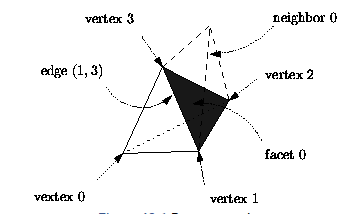
\includegraphics[width=0.5\textwidth]{figures/tetrahedron_cgal.png}
  \caption{Structure d'un tetrahèdre dans CGAL \cite{CGAL}}
  \label{fig::tetrahedron_cgal}
\end{figure}

Un tétrahèdre est représenté par quatre entités :
\begin{itemize}
  \item Vertex (sommet) : contient un point (coordonnées 3D)
  \item Cell (cellule) : un tétrahèdre qui donne accès à quatre sommets et quatre cellules adjacentes (les
  cellules qui ont une face commune avec la cellule courante)
  \item Edge (arête) : une arête contenant deux sommet ordonnés (l'arête va d'un point
  à un autre avec un sens établi) et une cellule
  \item Facet (face) : une face stockée grâce à une cellule et au sommet qui lui
  est opposé dans cette cellule
\end{itemize}

Il est important de comprendre la structure mise en place dans \gls{cgal} car il sera
nécessaire d'accéder aux différentes parties d'un tétrahèdre. Par exemple, lorsque
nous travaillons sur les arêtes pour rechercher l'interface, nous avons besoin de
connaître les sommets qui la composent.

Il existe également une seconde strucure de données, \textit{Polyhedron}, qui sera
utilisée pour stocker la surface. Cette classe permet de travailler sur des surfaces
en trois dimensions c'est-à-dire que les morceaux de cette surface sont en deux dimensions.
Le fonctionnement est sensiblement identique à la classe \textit{Delaunay\_Triangulation\_3}.
En effet, chaque polygone est également composé d'arêtes et de sommets auxquels on peut
accéder pour en récupérer les informations.

La compréhension des structures fournies par CGAL constitue donc une partie fondamentale du
projet. En effet la maîtrise des accesseurs (c'est-à-dire les méthodes qui permettent
d'accéder à chaque entité composant un térahèdre) est cruciale afin d'optimiser les parcours
dans les nuages de points via les itérateurs.





\subsection*{Itérateurs}

Les itérateurs sont une généralisation de pointeurs qui permettent de travailler sur
différentes structures de données. L'avantage est qu'ils sont liés aux différentes entités
qui composent un tétrahèdre. On peut comparer l'utilisation d'un itérateur à une boucle
\textit{for} dont l'ordre de parcours a été choisi au préalable afin d'optimiser
le temps de parcours.
Il existe des itérateurs permettant de parcourir une triangulation de Delaunay
selon chacune des entités formant celle-ci : vertice, arête, face, cellule. Quelle
que soit l'entité utilisée, il est possible d'accéder aux trois autres entités et
aux données qu'elles contiennent. Les itérateurs fonctionnent dans CGAL grâce aux
\textit{Handles}. Celles-ci sont des références indirectes qui fonctionnent sensiblement
comme des pointeurs. Lorsqu'on itère sur un des types composant les tétrahèdres, une
\textit{Handle} vers le type concerné est renvoyée. Par exemple, pour une itération sur des
vertices, on peut accéder à l'indice stocké dans \textit{info()} par la commande
fournie en figure \ref{fig::access_it}.

\begin{figure}[ht]
\centering
  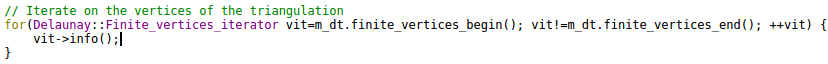
\includegraphics[width=\textwidth]{figures/access_it.png}
  \caption{Utilisation d'un itérateur}
  \label{fig::access_it}
\end{figure}


Il existe également des circulateurs qui, bien que semblables aux itérateurs par le fait
qu'ils parcourent des structures de données, fonctionnent différemment. Comme leur nom
l'indique, ils permettent de "tourner" autour d'une entité. Par exemple ils peuvent
servir à parcourir toutes les cellules adjacentes d'une cellule donnée. Ils s'utilisent
sous la forme d'une boucle \textit{do...while} (voir figure \ref{fig::circ_ex}).
\begin{figure}[ht]
\centering
  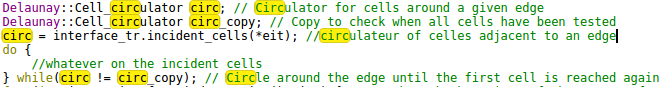
\includegraphics[width=\textwidth]{figures/circ_ex.png}
  \caption{Utilisation d'un circulateur}
  \label{fig::circ_ex}
\end{figure}
 Le circulateur est incrémenté à chaque
passage dans la boucle jusqu'à ce qu'il soit revenu à son point de départ. Il aura alors
effectué un "tour" complet autour de l'entité de notre choix.


Nous verrons, lors de l'implémentation, qu'un bon usage des circulateurs, et plus encore des itérateurs,
est absolument crucial pour l'optimisation des temps de parcours et la validité
des résultats obtenus. Ils permettent également de rendre le code plus générique.

Nous verrons également comment la méthode théorique a été implémentée grâce en partie à CGAL
dans la suite de notre projet.
